\documentclass{article}
\usepackage[utf8]{inputenc}
\usepackage{graphicx}
\usepackage{ccicons}

\title{\textbf{Introduction to Overleaf}}
\author{Anna Volkova \& Marco Schirone}
\date{February 2021}

\usepackage[english]{babel}
\usepackage[style=ieee]{biblatex} 
% Try to change the reference style to APA Style with \usepackage[style=apa]{biblatex} or to the Vancouver Style with \usepackage[style=vancouver]{biblatex} 

\addbibresource{references.bib} %Imports bibliography file

\usepackage{hyperref}
\usepackage{csquotes}

\begin{document}
\maketitle

\section{Introduction}
Thank you for joining the session! Please find some helpful links below.


\begin{figure}[h!]
\centering
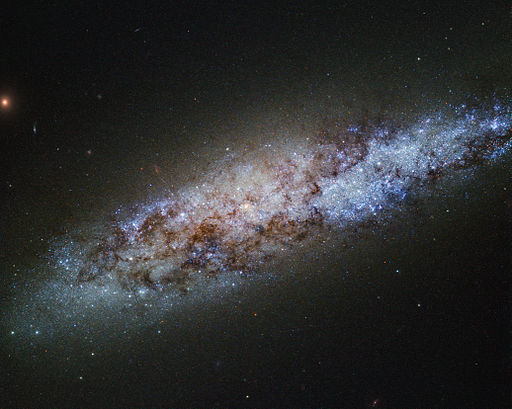
\includegraphics[scale=0.3]{universe}

\caption{The Universe. CC-BY 4.0 ESA/Hubble}\ccby
\label{fig:universe}
\end{figure}


\section{Helpful Links}
\begin{itemize}
\item{Chalmers Library}

    \begin{itemize}
    \item {\href{http://www.lib.chalmers.se/en/}{Chalmers Library}}
    \item {\href{https://guides.lib.chalmers.se/overleaf_latex}{Overleaf Guide from Chalmers Library}}
    \item {\href{https://guides.lib.chalmers.se/reference_management_software}{Reference Management Software}}
    \end{itemize}  

\end{itemize}

\begin{itemize}
\item{Overleaf}

 \begin{itemize}  
    \item {\href{https://www.overleaf.com/latex/templates/a-quick-guide-to-latex-overleaf-version/bphpqrdgjyqy}{A Quick Guide to LaTeX}}
    \item {\href{https://www.overleaf.com/articles/overleaf-keyboard-shortcuts/qykqfvmxdnjf}{Overleaf Keyboard Shortcuts}}
    \item {\href{https://www.overleaf.com/learn/latex/Learn_LaTeX_in_30_minutes}{Learn LaTeX in 30 Minutes}}
    \item {\href{https://www.overleaf.com/events/webinars}{Overleaf Webinars}}
\end{itemize}
 \end{itemize}


\section{Conclusion}

``I always thought something was fundamentally wrong with the universe'' \cite[ p. 12]{adams}

\printbibliography
\end{document}
